Il package \textit{gamelogic} rappresenta il model, ovvero la logica del gioco, e si compone di:

\begin{itemize}
    \item \textbf{Arena}: Questa classe contiene le entità che popolano la mappa in un dato momento della partita, nonchè tutti i metodi necessari per interagire con esse e l'area di gioco. Volendo accedere allo stato della partita in corso, infatti, basterà controllare lo stato delle strutture dati per le entità. Una funzione \textit{generateMap()} viene richiamata, attraverso il controller, nella fase di popolazione iniziale, ovvero all'inizio di ogni livello, e una funzione \textit{updateMap()} invece si occupa dell'aggiornamento dello stato di ogni entità e viene richiamata ad ogni step logico, come si può vedere dal codice in figura \ref{arenaCode}.
    
    \begin{figure}[H]
        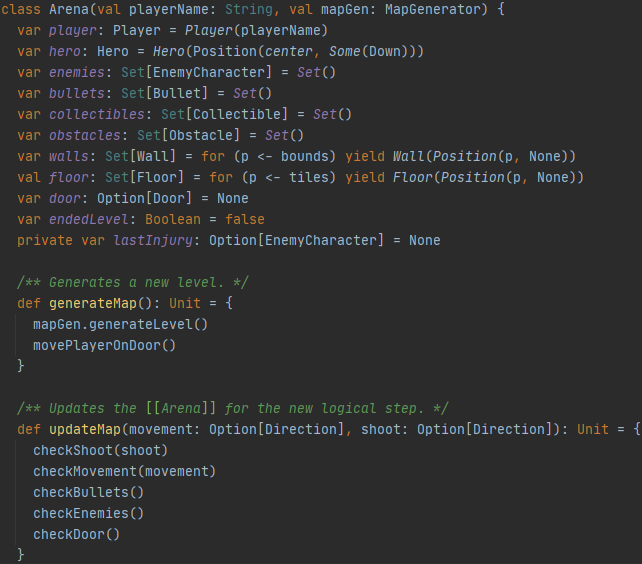
\includegraphics[width=15cm]{res/arenaCode.png}
        \caption{Esempio di codice di \textit{Arena}}
        \label{arenaCode}
    \end{figure}
    
    \textit{MapGenerator} (figura \ref{mapGeneratorCode}), facente parte dei parametri di inizializzazione della classe, incapsula la logica di generazione a partire dalla difficoltà scelta. Implementa il legame tra la difficoltà del gioco (rappresentata da un insieme di valori e range) ed il modo randomico con cui vengono generate le entità.
    
    \begin{figure}[H]
        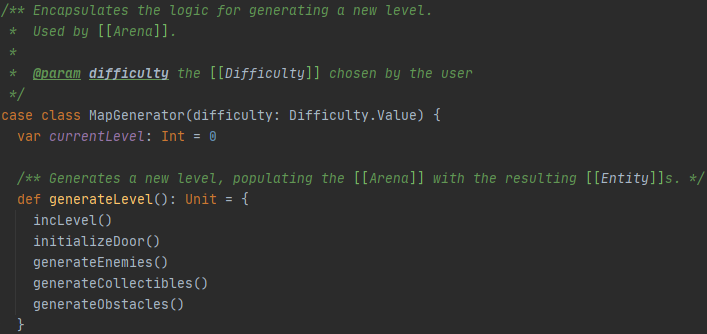
\includegraphics[width=15cm]{res/mapGeneratorCode.png}
        \caption{Esempio di codice di \textit{MapGenerator}}
        \label{mapGeneratorCode}
    \end{figure}

    \item \textbf{GameState}: Un object che incapsula lo stato attuale della partita. La classe \textit{Arena} viene istanziata al suo interno, rendendolo il punto di riferimento per avere accesso al contesto del gioco. Infatti, il controller ne richiama i metodi che incapsula per la gestione della partita, come ad esempio l'avvio del gioco, il richiamo dello step da eseguire, la generazione di un nuovo livello e la gestione dei record.
    
    \item \textbf{Entity}: Come riportato in figura \ref{model}, tutti gli elementi del gioco estendono da questa interfaccia. Il trait \textit{Entity} rappresenta una qualsiasi entità sulla mappa di gioco, dotata di una posizione propria. Viene poi esteso per distinguere tra le entità che occupano una posizione fissa (\textit{Collectible}, \textit{Obstacle}, componenti dell'arena) e quelle che invece possono muoversi (\textit{MovableEntity}): queste ultime possiedono metodi per avanzare di posizione all'interno dell'arena, data una direzione di movimento. Il trait \textit{EnemyCharacter} rappresenta i nemici, mentre il trait \textit{LivingEntity} viene applicato alle entità dotate di un proprio punteggio che ne rappresenta la vita a disposizione (\textit{Hero}, \textit{EnemyCharacter}).
\end{itemize}

\begin{figure}[H]
  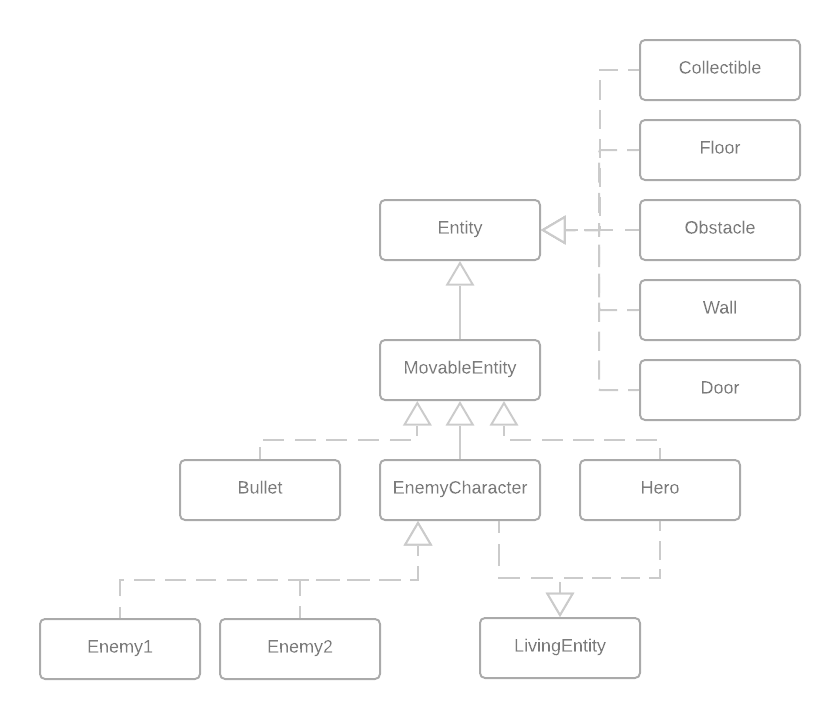
\includegraphics[width=14cm]{res/GAMELOGIC_Diagram.png}
  \caption{Organizzazione della logica di gioco}
  \label{model}
\end{figure}